% !TEX root = ../../../main.tex
% 来源：中学数学实验教材·第二册（几何）
% 章节：实验几何 / 基本作图
% 原始文件：1.tex，行 3467-3484
% 类型：tikz
% ---
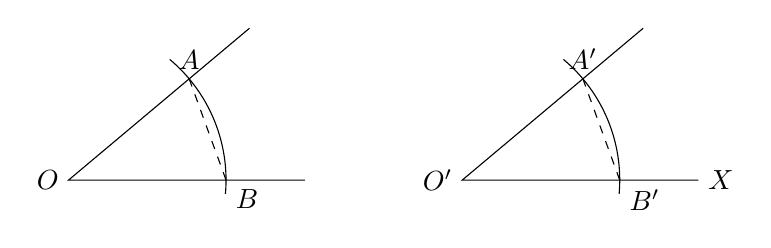
\begin{tikzpicture}
\begin{scope}
\draw(40:3)--(0,0)node[left]{$O$}--(3,0);
\draw(-5:2) arc (-5:50:2);
\node at (40:2)[above]{$A$};
\draw[dashed](2,0)node[below right]{$B$}--(40:2);
\end{scope}
\begin{scope}[xshift=5cm]
	\draw(40:3)--(0,0)node[left]{$O'$}--(3,0)node[right]{$X$};
	\draw(-5:2) arc (-5:50:2);
	\node at (40:2)[above]{$A'$};
	\draw[dashed](2,0)node[below right]{$B'$}--(40:2);
\tkzDefPoint(2,0){B'}
\tkzDefPoint(40:2){A'}
\tkzCompass[color=black](B',A')

\end{scope}
\end{tikzpicture}
